\documentclass[10pt,a4paper]{article}
\usepackage[utf8]{inputenc}
\usepackage[italian]{babel}
\usepackage{amsmath}
\usepackage{amsfonts}
\usepackage{amssymb}
\usepackage{graphicx}
\usepackage[left=2cm,right=2cm,top=2cm,bottom=2cm]{geometry}
\newcommand{\rem}[1]{[\emph{#1}]}

\author{Gruppo AC \\ Federico Belliardo, Francesco Mazzoncini, Giulia Franchi}
\title{Esercitazione N.2: Circuito RC - Filtri Passivi.}
\begin{document}

\maketitle

Tanti auguri!

\section{Scopo e strumentazione}

Misurare la frequenza di un filtro passa-basso e studiare la variazione della risposta del filtro in funzione del carico applicato a valle. In seguito studiare la l'attenuazione di un filto passa-banda.

\section{Filtro passa-basso}
\paragraph{Progettazione filtro}
Si vogliono trovare i valori dei componenti resistivo e capacitivo del filtro perchè trasmetta un segnale sinusoidale di frequenza $2kHz$ e attenui il rumore a $20kHz$.

\begin{figure}[h]
\centering
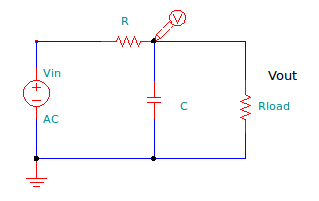
\includegraphics[scale=1.0]{passabasso.png}
\caption{Schema del circuito passa-basso}
\end{figure}

Risolvendo il circuito e chiamando $r$ la resitenza di carico e $R$ la resistenza del passabasso si ottiene la seguente relazione per il modulo dell'attenuazione:
$\vert A(\omega) \vert = \frac{1}{\sqrt{(1+x)^2+(\frac{f}{f_{0}})^2}} $. Dove $f_0$ è la frequenza di taglio del filtro. Definite $f_2 = 20 kHz$ e $f_1 = 2 kHz$ le freuenze del rumore e del segnale e $x = \frac {R}{r}$ otteniamo come rapporto di attenuazione: 
$\vert \frac{A(2 kHz)}{A(20 kHz} \vert = \sqrt{\frac{{f_0}^2 (1+x)^2 + {f_2}^2}{{f_0}^2 (1+x)^2 + {f_1}^2}}$

Selezionando una resistenza $R = 1 k\Omega$ del filtro molto minore del carico $r = 100 k\Omega$ otteniamo $x = 0.01$ cioè un valore per x trascurabile e possiamo scrivere (le unità sono state prese $kHz$): 
$\vert \frac{A(2 kHz)}{A(20 kHz} \vert = \sqrt{\frac{{f_0}^2  + 400}{{f_0}^2 + 4}}$. Con n condensatore $C = 80 nF$ si ottiene una rapporto segnale rumore $\vert \frac{A(2 kHz)}{A(20 kHz} \vert \sim 7$ e una attenuazione del segnale $\vert A(2 kHz) \vert \sim \frac{1}{\sqrt{2}}$.

Abbiamo a disposizione un condensatore da $C = \pm nf$, e questo implica avere una resistenza $R = \pm k\Omega$.
La frequenza di taglio quindi è $f_0 = \pm kHz$ e da questi valori stimiamo i valori di $\vert A(2 kHz) \vert = \pm $ e di $\vert \frac{A(2 kHz)}{A(20 kHz} \vert$.

\paragraph{Misura frequenza di taglio}

Si è misurata la frequenza di taglio dall'intersezione delle due rette del fit. Chiamate le rette $y = a_1 x+b_1$ e $y = a_2 x+b_2$, il loro punto di intersezione è $f_0 = (b_1 - b_2)/(a_1 - a_2)$. 

\paragraph{Impedenza del circuito a bassa frequenza}
L'impedenza di ingresso di un circuito come quello disegnatio all'inizio della relazione è $Z_ingresso = R+\frac{r}{j \omega C r+1}$ , dunque a bassa frequenza in condensatore è un aperto dunque l'impedenza di ingresso è $R+r$, mentre ad alta frequenza è un cortocircuito dunque l'impendenza è $R$. Alla frequenza di taglio abbiamo poi: $Z_ingresso = R + \frac{Rr}{jr+R}$. L'efetto della resistenza di carico sul circuito è di diminuirne il guadagno, secondo la formula: $\vert A(\omega) \vert = \frac{1}{\sqrt{(1+x)^2+(\frac{f}{f_{0}})^2}} $.
Lo scostamento della risposta da quella del filtro ideale è tanto maggiore quanto il carico resistivo è più vicino alla resistenza del filto.

\section{Filtro passa-banda}

\begin{figure}[h]
\centering
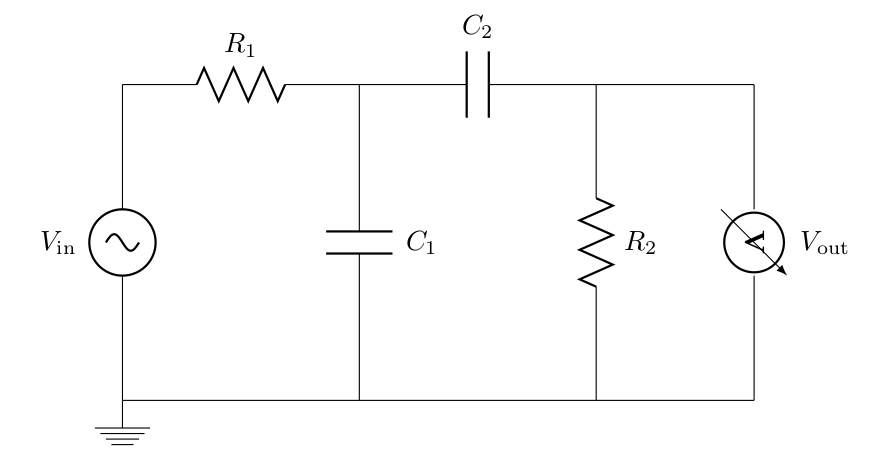
\includegraphics[scale=0.4]{passabanda.png}
\caption{Filtro passa banda}
\end{figure}

\paragraph{Verifiche sui circuiti passa alto e passa basso}

\paragraph{Misure sul fitro passa banda}
%misure delle frequenze di taglio e dell'ampiezza massima (dovrebbe essere -6 dB)

\paragraph{Spegazioni teoriche}
La funzione di trasferimento teorica per un circuito passa banda come quelli disegnati sopra è: 
$V_{out} = A_{1} A_{2} \frac{Z_{in}^2}{Z_{out}^2+Z_{in}^2} V_{in}$, dove gli apici si riferiscono a al primo o al secondo circuito in sequenza. 

La seguente tabella riassume le impedenze di ingresso e sucita per circuiti passa basso:

\begin{table}[h]
\centering
\begin{tabular}{|c|c|c|}
\hline 
 & Passa-basso  & Passa-alto \\
\hline 
Ingresso & $R+\frac{1}{j \omega C}$ & $R+\frac{1}{j \omega C}$\\ 
Uscita & $AR$ & $j \omega C A$\\
\hline 
\end{tabular} 
\caption{Riassunto resistenze di ingresso e di uscita.}
\end{table}

Semplificando l'espressione otteniamo: $V_{out} = A_{1} A_{2} \frac{1}{1+\frac{R_1}{R_2} A_1 A_2} V_{in}$.
E nel nostro caso (due resistenze uguali otteniamo:
$V_{out} = A_{1} A_{2} \frac{1}{1+A_1 A_2} V_{in}$, che è limitato dall'alto da $A_{max} = \frac{1}{2}$.
Se chiamiamo $\omega_1$ la frequenza di taglio del circuito passa alto e $\omega_2$ la frequenza di taglio del circuito passa alto e la frequenza del cicruito passa basso otteniamo i seguenti limiti per l'attenuazione:
\begin{itemize}
\item $\omega \ll \omega_1$ allora $A_1 \sim 1$ dunque 
$A_{tot} = \frac{A_2}{1+A_2}$, sviluppando otteniamo 
$A_{tot} = \frac{1}{2} \frac{1}{1-j \frac{\frac{\omega_2}{2}}{\omega}}$ dunque il filtro è equivalente a un passa alto con frequenza di tagio $\frac{\omega_2}{2}$. 
\item $\omega \gg \omega_2$ allora $A_2 \sim 1$ dunque 
$A_{tot} = \frac{A_1}{1+A_1}$, sviluppando otteniamo:
$A_{tot} = \frac{1}{2} \frac{1}{1+j \frac{omega}{2 \omega_1}}$.
\end{itemize}

Se vogliamo che $A_{tot} = A_1 A_2$ deve essere $R_1 \ll R_2$ come è evidente.

\end{document} 